\section{Defining Safety Specifications for Synchronous Neural Networks}
\label{sec:definitions}

We propose the use of bi-directional run-time enforcers~\cite{recps} to enforce the I/O events of \acp{SNN} at run-time.
In order to specify the safety policies Pinisetty et al define \acf{DTA}~\cite{recps}.
These \ac{DTA} can enforce binary events at run-time using \textit{edit functions}~\cite{recps}.
To enforce the policy $\varphi$, the run-time enforce must satisfy some constraints: soundness, monotonicity, instantaneity, transparency and causality.
The enforcers by \cite{recps} were demonstrated to satisfy all above constraints.

However, with the complex I/O of \acp{SNN}, an enforcer that edits only binary events is not sufficient.
Additionally, the edit functions introduced by \cite{recps} are not sufficient with more complex \ac{DTA}.

\begin{figure}[H]
	\centering
	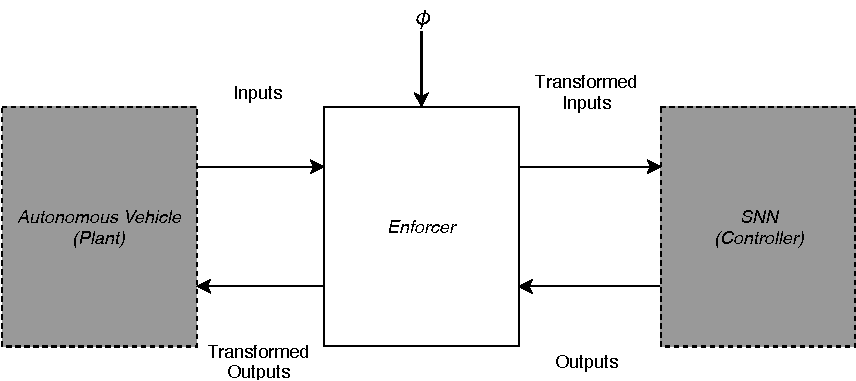
\includegraphics[width=0.8\linewidth]{Content/Fig/RE.pdf}
	\caption{Run-time enforcer between a \ac{SNN} and the \acf{AV}, to monitor the I/O events of the \ac{SNN}. \label{fig:re}}
\end{figure}

Consider Figure~\ref{fig:re}, we wish to enforce the inputs and outputs events of the \ac{SNN}, defined by some safety policy $\varphi$.
However, the outputs from the \ac{SNN} are 32-bit integer values, i.e. we cannot use a \ac{DTA} to to specify the safety policies for this \acp{SNN}.
We propose the use of \acfp{VDTA} to enforce valued I/O events of \acp{SNN}. 

\subsection{\acf{VDTA}: Defining Safety Policies for \ac{CPS}}

We consider our industrial \ac{CPS} systems to have finite ordered sets of valued input channels ${I} = \{{i_1}, {i_2}, \ldots {i_n}\}$ and valued output channels ${O} = \{{o_1}, {o_2}, \ldots {o_n}\}$.

A VDTA can be seen as a DTA with a finite set of locations, a finite set of discrete clocks used to represent time evolution, and external input (resp. output channels) called ``external variables'' which are used for representing system data.
They also have internal variables which are used for internal computation, compared to the external variables which model the data carried by the actions from the monitored system (resp. environment). 
In a VDTA, a transition consists of an action carrying values of external variables, a guard on internal variables, external variables and clocks, and an assignment of internal variables, and reset of clocks.
%Thus, each input (resp. output channel) is considered as an external variable. 

Before we look into the formal definition of VDTA, let us consider an example.

\begin{figure}[H]
	\centering
	\includegraphics[width=0.7\linewidth]{avpedrte.tikz}
	\caption{\ac{VDTA} for describing the safety policy for the pedestrian detection $\mathcal{V}_{ped}$\label{fig:avpedrte}}
\end{figure}

\begin{example}
	The case study can be presented by four, different \acp{VDTA}; $\mathcal{V}_{ped}$, $\mathcal{V}_{car}$, $\mathcal{V}_{drive}$ and $\mathcal{V}_{cnn}$, as depicted in Figures~\ref{fig:avpedrte}, \ref{fig:avcarrte}, \ref{fig:avdriverte} and \ref{fig:avcnnrte} respectively. 
	For the purposes of these examples, the \ac{VDTA} for the pedestrian safety policy, $\mathcal{V}_{ped}$, is used.
	This \ac{VDTA} specifies that driving towards a pedestrian in-front of the vehicle and not braking is a violation, and approaching a pedestrian from a distance and not starting to slow down is also violation.
	I.e. taking any action which may endanger surrounding pedestrians is in violation to the safety policy.
	
	This is encoded as a \ac{VDTA} with a set of locations $L = \{l_{drive}, l_{brake}, l_v\}$ and accepting locations $F = \{l_{drive}\}$, with the initial state being $l_{drive}$.
	The set of external variables $C = \{O_2, O_5, O_{2_v}, O_{5_v}, S, A, B_S, B_H\}$ are all 32-bit signed integers, where $O_2$, $O_5$, $O_{2_v}$, $O_{5_v}$ and $S$ are input channels and $A$, $B_S$ and $B_H$ are output channels.
	The set of actions $\Sigma = \{tk(O_2, O_5, O_{2_v}, O_{5_v}, S, A, B_S, B_H)\}$, and the set of internal variables $V = \{T_{lim}\}$, where $T_{lim}$ is a 32-bit signed integer.
	In the example, $\tau$ is a function with $O_2$, $O_5$, $O_{2_v}$, $O_{5_v}$ and $S$ as input parameters. 
	
	In this \ac{VDTA} there are two violation transitions, labelled \textcircled{a} and \textcircled{b} in Figure~\ref{fig:avpedrte}.
	\textcircled{a} occurs when the vehicle does anything else other than braking when there is a pedestrian in-front or not braking when there is no pedestrian ahead of the vehicle.
	\textcircled{b} can also occur when the vehicle has not braked enough within a certain period of time $T_{lim}$, or when the vehicle remains braking longer than is safe or necessary.
	This represents the vehicle taking further unsafe actions when already in an unsafe state.
\end{example}


Let us now consider in more detail the formal syntax and semantics of VDTAs.
%
For a variable (resp. channel) $v$, ${\cal D}_v$ denotes its domain,
and for a tuple of variables $V= (v_1, \ldots, v_n)$,
${\cal D}_V$ is the product domain ${\cal D}_{v_1} \times \cdots \times {\cal D}_{v_n}$.
%A predicate $P(V)$ on a tuple of variables $V$ is a logical formula whose semantics is a function ${\cal D}_V \rightarrow \{\true, \false\}$.
A valuation of the variables in $V$
is a mapping $\nu$ which maps every variable $v \in V$ to a value $\nu(v)$ in ${\cal D}_v$.
%
Let $X=\{x_1,\ldots, x_k\}$ be a finite set of integer variables representing discrete clocks.
%
A {\em valuation} for $x$ is an element of $\bbn$, that is a function from $x$ to $\bbn$.
The set of valuations for the set of clocks $X$ is denoted by $\chi$.
%
For $\chi\in\bbn^X$, $\chi+1$ (which captures the ticking of the digital clock) is the valuation assigning $\chi(x)+1$ to each clock variable $x$ of $X$.
Given a set of clock variables $X' \subseteq X$, $\chi[X' \leftarrow 0]$ is the valuation of clock variables $\chi$ where all the clock variables in $X'$ are assigned to $0$.

\begin{definition}[Syntax of {VDTA}s]
	\label{def:ptav}
	A {VDTA} is a tuple \\
	$\calA = \left(\Sigma, L, {l_0}, X, V, C, \Theta, F,  \Delta \right)$ where:
	\squishlist
	\item $\Sigma$ is a non-empty finite set of actions,
	and an action $a \in \Sigma$ has a signature $sig(a) = ( t_0, t_1, \ldots, t_k )$ which is a tuple of types of the external variables,
	\item $L$ is a finite non-empty set of locations, with $l_0 \in L$ the initial location, and $F \subseteq L$ the set of accepting locations;
	\item $X$ is a finite set of discrete clocks;
	\item $V$ is a tuple of typed internal variables; 
	\item $C$ is a tuple of external variables, where $C = I \cup O$, where $I$ is the set of input channels, and $O$ is the set of output channels; 
	\item $\Theta\subseteq {\cal D}_{V }$ is an initial condition which is a computable predicate over $V$;
	\item $\Delta$ is a finite set of transitions, and each transition $t \in \Delta$ is a tuple $( l, a, c, G, A, l' )$
	also written\\
	$l \xrightarrow{a(c), G(V,c), V':=A(V,c)} l'$
	such that,
	\squishlist
	\item[\textbullet] $l, l' \in L$ are respectively the origin and target locations of the transition;
	\item[\textbullet] $a \in \Sigma$ is the action, and $c=( c_1, \ldots c_k )$ is a tuple of external variables local to the transition;
	\item[\textbullet] $G = G^D \wedge G^X$ is the guard where
	\squishlist
	\item[-] $G^D \subseteq {\cal D}_V \times {\cal D}_{sig(a)}$
	is a computable predicate over internal variables and external variables  in $V \cup c$;
	\item[-] $G^X$ is a clock constraint over $X$ defined as a Boolean combinations of constraints of the form $x \sharp f(V \cup c)$, where $x \in X$ and $f(V \cup c)$ is a computable function, and $\sharp \in \{ <, \leq, =, \geq, > \}$;
	\squishend
	\item[\textbullet] $A$$=$$(A^D, A^X)$ is the assignment of the transition where
	\squishlist
	\item[-] $A^D :{\cal D}_V \times {\cal D}_{sig(a)} \rightarrow {\cal D}_V$ defines the evolution of internal variables.
	\item[-] $A^X \subseteq X$ is the set of clocks to be reset.
	\squishend
	\squishend
	\squishend
\end{definition}
%
A word is a sequence $\sigma = e_1\cdot e_2 \cdots e_n$ where $\forall i \in [1,n]: e_i = a_i(\eta_i)$ where $a_i \in \Sigma$ is an action and $\eta_i \in {\cal D}_V$ is a vector of values of a tuple of variables $V$. 

Policy \ac{VDTA} are required to be \textit{deterministic}, i.e. for any given state, the conjunction of any guards of any other outgoing transitions may not be satisfiable; and \textit{complete}, i.e. for any given state at any given time and any given event, at least one transition guard is satisfied.

\subsection{Semantics for \ac{VDTA}}

Let $\calA = \left(\Sigma, L, {l_0}, X, V, C, \Theta, F,  \Delta \right)$  be a VDTA.
The semantics of $\calA$ is a timed transition system,
where a state consists of a location, and valuations of internal variables $V$ and clocks $X$, and actions associated with values of external variables in $C$.

\begin{definition}[Semantics of {VDTA}s]
	\label{def:vdta:semantics}
	The semantics of $\calA$ is a timed transition system $\sem{\calA}=( Q, q_0, Q_F, \Gamma, \to )$, defined as follows:
	\squishlist
	\item $Q = L \times {\cal D}_V \times \bbn^X$, is the set of states of the form $q= ( l,\nu ,\chi )$ where
	$l \in L$ is a location,
	$\nu \in {\cal D}_V$ is a valuation of internal variables,
	$\chi$ is a valuation of clocks;
	\item $Q_0 = \{ ( l_0,\nu, \chi_{[X \leftarrow 0]} )  \mid \Theta(\nu)=\true \}$ is the set of initial states;
	\item $Q_F = F \times {\cal D}_V \times \bbn^X$ is the set of accepting states;
	\item $\Gamma = \{ a(\eta) \mid
	a \in \Sigma \wedge \eta \in {\cal D}_{sig(a)}  \}$ is the set of transition labels;
	\item $\to\subseteq Q\times \Gamma\times Q$  the transition relation
	is the smallest set of transitions of the form
	$( l,\nu,\chi \rangle \longrightarrow {a(\eta)} \langle l',\nu',\chi')$
	such that  $\exists ( l, a, c, G, A, l' ) \in \Delta$,
	with $G^X(\chi + 1) \wedge G^D(\nu, \eta) $ evaluating to {\true},
	$\nu'= A^D(\nu, \eta)$ and $\chi'=(\chi+1)[A^X \leftarrow 0]$.
	\squishend
\end{definition}


%The set of timed words over $\Sigma$ where the actions carry parameter value and other data is denoted by $\tw(\Lambda)$.
A {\em run} $\rho$ of $\sem{\calA}$ from a state $q\in Q$ over a {\em trace} $w =  a_1(\eta_1)\cdot a_2(\eta_2)\cdots a_n(\eta_n)$ is a sequence of moves in $\sem{\calA}$:
$\rho = q \xrightarrow {a_1(\eta_1)} q_1
\cdots q_{n-1}\xrightarrow {a_n(\eta_n)} q_{n}$,
for some $n\in\bbn$.
The set of runs from the initial state $q_0\in Q$,  is denoted $\Run(\calA)$ and $\Run_{Q_F}(\calA)$ denotes the subset of those runs {\em accepted} by $\calA$, i.e.,  ending in an accepting state $q_n \in Q_F$.

%%%%%%%%%%%%%%%%%%%%%%%%%%%%%%%%%%%%%%%%%%%%%%%
%%%%%%%%%%%%%%%%%%%%%%%%%%%%%%%%%%%%%%%%%%%%%%%
\ignore{
\begin{example}[Run of a VDTA]
	Let us consider the VDTA discussed in Example\ref{eg:vdta} presented in Figure~\ref{fig:vsa-overcurrent}. 
	An example run of the VDTA depicted in Figure~\ref{fig:vsa-overcurrent} is elaborated here.
	Let the internal variable $i_{max}$ be initialized with 10000.
	A run of this VDTA starting from the initial state $(l_{safe}, i_{max}=10000, x = 0)$ for the word $\sigma = tk(4000, 5000,1)\cdot tk(8000, 5000,1)\cdot tk(7000, 5000,1)\cdot tk(8000, 5000,1)\cdot tk(8000, 5000,1)\cdot tk(8000, 5000,1)$ is given below:\\
	$
	(l_{safe}, i_{max}=10000, x = 0)
	\xrightarrow {tk(4000, 5000,1)} \\
	(l_{safe}, i_{max}=10000, x = 1)
	\xrightarrow {tk(8000, 5000,1)} \\
	(l_{unsafe}, i_{max}=10000, x = 0)
	\xrightarrow { tk(7000, 5000,1)} \\
	(l_{unsafe}, i_{max}=10000, x = 1)
	\xrightarrow { tk(8000, 5000,1)} \\
	(l_{unsafe}, i_{max}=10000, x = 2)
	\xrightarrow { tk(8000, 5000,1)} \\
	(l_{unsafe}, i_{max}=10000, x = 3)
	\xrightarrow { tk(8000, 5000,1)} \\
	(l_{vio}, i_{max}=10000, x = 4).
	$
	
	The run started in the initial state and ended in a non-accepting state. It is thus a non-accepting run and represents a violation scenario.
}


\begin{example}[Run of a VDTA]
	\label{ex:run}
	An example run of the VDTA presented in Figure~\ref{fig:avpedrte} is presented here.
	Assume that the time the vehicle has to be braking is $T_{lim} = 2$. 
	The starting state is $l_{drive}$, and the first I/O event is $(\{0, 0, 0, 0, 4063232\}, \{\langle 0, 0, 0 \rangle\})$, i.e. nothing is detected in-front of the vehicle and the vehicle does not accelerate or brake, meaning it is cruising at 62 km/h.
	Thus, the automaton remains in state $l_{drive}$.
	Next tick, $(\{0, 65536, 0, 655360, 4063232\}, \{\langle 0, 65536, 0 \rangle\})$ occurs, i.e. a pedestrian is detected quite far ahead of the vehicle, moving across the road at 10 km/h, and the vehicle is taking a soft braking action from 62 km/h.
	Since ${O} = \{\langle 0, 65536, 0 \rangle\}$ which is a soft brake $B_S$ and Object 5, far ahead of the vehicle, is a pedestrian $O_5 = 65536 = O_{5_P}$ the system enters the unsafe state $l_{brake}$ and $t = 0$ is set.
	Then,  $(\{65536, 0, 0, 0, 2621440\}, \{\langle 0, 0, 0 \rangle\})$ is received, i.e. the pedestrian has stopped moving in the road and is now close to the vehicle, however the vehicle is not braking, but rather cruising at 40 km/h.
	Since no braking is detected, the violation transition $l_v$ is taken.
	As such, this run was \textit{non-accepting}.
\end{example}

\subsection{Defining Safety Automata for an \ac{AV} system}
In order for the \ac{AV} system to operate safely, it must follow a set of policies ($\mathcal{V}$), defined in English here:

$\mathcal{V}_{cnn}$ (Figure~\ref{fig:avcnnrte}): The output of the vision \ac{CNN} ensemble networks ($O$) must match the \ac{LiDAR} values ($L$) when the confidence of the ensemble networks is low. 
If the confidence is high, and there is a mismatch, the output should be classified as \textit{unknown} ($U$).
The system should treat this output as if it were a pedestrian, i.e. with utmost caution.

$\mathcal{V}_{drive}$ (Figure~\ref{fig:avdriverte}): The vehicle may not exceed the safe speed limit. 
An \textit{acceleration} command $A$ should be suppressed when the vehicle's speed limit of 100km/h is reached.

$\mathcal{V}_{car}$ (Figure~\ref{fig:avcarrte}): Ensure that the car does not drive into other vehicles. If an \textit{acceleration} command $A$ is asserted when the car in front (i.e. $O_{2_C}$ or $O_{5_C}$) is driving slower than the \ac{AV} ($O_{2_V}<S|O_{5_V}<S$), then this is suppressed and instead an appropriate brake speed $B_S$ (soft) or $B_H$ (hard) would be asserted instead.

$\mathcal{V}_{ped}$ (Figure~\ref{fig:avpedrte}): Ensure that the car does not behave unsafely around pedestrians. If a pedestrian appears in-front of the vehicle $P=true$, then the car should select an appropriate braking action (either $B_S$ or $B_H$). If a pedestrian remains off to the side of the vehicle, then either the vehicle should cruise or a braking action is appropriate.

\begin{figure}[H]
	\centering
	\includegraphics[width=0.5\linewidth]{avcarrte.tikz}
	\caption{\ac{VDTA} for describing the safety policy for the car detection $\mathcal{V}_{car}$\label{fig:avcarrte}}
\end{figure}
\begin{figure}[H]
	\centering
	\includegraphics[width=0.5\linewidth]{avdriverte.tikz}
	\caption{\ac{VDTA} for describing the safety policy for driving according to the rules $\mathcal{V}_{drive}$\label{fig:avdriverte}}
\end{figure}
\begin{figure}[H]
	\centering
	\includegraphics[width=0.5\linewidth]{avcnnrte.tikz}
	\caption{\ac{VDTA} for describing the safety policy for the \ac{CNN} ensembles $\mathcal{V}_{cnn}$\label{fig:avcnnrte}}
\end{figure}

We can define these rules of the \ac{AV} system as a \textit{Safety Automata}~\cite{recps}, which are a kind of \acf{DTA}. 
Examples of this are presented in Figures \ref{fig:avpedrte} - \ref{fig:avcnnrte}, which represent the automata used in the four policies of the \ac{AV} system.
%Here, $A$ refers to the accelerate action, $B_S$ refers to a slow, or gentle, braking action, $B_H$ refers to a hard braking action.
$P$ is a flag that denotes the presence of a pedestrian in a position that will be dangerous at any point in the future, and $t$ is a timer that ensures that the \ac{AV} has braked for long enough and in time when a collision with a pedestrian has been detected, denoted by the time $T_{lim}$. 
$T_{lim}$ is a predefined length of time by which the system should have reacted to a pedestrian in a dangerous position.

Finally, a complete policy framework can be established by simply ANDing the component policies together, i.e. \\ $\mathcal{V}_{av} = \mathcal{V}_{cnn} \wedge \mathcal{V}_{drive} \wedge \mathcal{V}_{car} \wedge \mathcal{V}_{ped}$.

%The first policy, $\mathcal{V}_{cnn}$, compares the \ac{LiDAR} depiction and the classified image class from the corresponding ensemble outputs, if the \ac{LiDAR} and ensemble outputs are different, and the ensemble confidence value is low, the ensemble output is changed to match the output of the corresponding \ac{LiDAR} reading.
%If the ensemble confidence is high, both the \ac{LiDAR} reading and the corresponding ensemble output are changed to signal that the object detected is \textit{Unknown} and should be treated with extra caution, as if the object were a pedestrian.
%The second policy, $\mathcal{V}_{drive}$, ensures that the vehicle maintains reasonable driving practices on the road, e.g. not staying stationary in the middle of the road and not speeding.
%If the \ac{AV} controller outputs that the \ac{AV} should \textbf{accelerate} while the \ac{AV} is at the speed limit, the \textbf{accelerate} command would be changed to a  \textbf{cruise} command.
%Likewise, if the \ac{AV} controller decides that the \ac{AV} should remain stationary in an empty road, the \textbf{brake} (or \textbf{cruise}) command would be modified to an \textbf{accelerate} command.
%The third policy, $\mathcal{V}_{car}$, checks the environment for other vehicles and ensures that the \ac{AV} does not drive into other vehicles, or cause accidents with other vehicles in any way.
%If the \ac{AV} would \textbf{accelerate} into a vehicle in front, the \textbf{accelerate} would be changed to a \textbf{cruise}, if the \ac{AV} was driving much faster than the vehicle in front and the \ac{AV} is not braking, the current action would be modified to be a \textbf{brake} action.
%The fourth, and highest priority, policy ($\mathcal{V}_{ped}$) monitors the environment for pedestrians and ensures that the car does not exhibit unsafe behaviour with regards to the pedestrians. 
%If the \ac{AV} were to \textbf{accelerate}, or \textbf{cruise}, into a pedestrian that is in front of the vehicle, or approaching the road from the sides, the \textbf{accelerate}, or \textbf{cruise}, action would be changed to a \textbf{brake} action.
%If the \ac{AV} does not brake fast enough with a pedestrian in front of the \ac{AV}, or approaching from the sides, a \textbf{hard brake} action would be initiated instead of the \ac{ANN} proposed action.
%This policy ensures that the vehicle always drives slowly and cautiously around pedestrians.


\subsection{Enforcing Non-accepting I/O Events}
Enforcers are designed to prevent a system from generating an input/output trace that is non-accepting, such as Example~\ref{ex:run}.
\cite{recps} proposed \ac{DTA} semantics with two possible methodologies for editing non-accepting I/O events.
These are \textit{random} and \textit{minimum} edits; a random edit chooses a random, accepting event from a list of accepting I/O events and minimum edit chooses the closest accepting event to the current non-accepting event.
However, neither of these edits are not always useful for problems in real scenarios.
Take Example~\ref{ex:run}, when the transition $l_{drive} \rightarrow l_v$ is taken, Object 2 can be edited such that $l_v$ is not entered, however this will not remove the danger that initially posed this transition.
However, if the action ${O}$ was changed, e.g. the cruising action in the example that caused the non-accepting trace was changed to a hard braking action, then an accepting event would have occurred \textit{and} the pedestrian in the road would have been safe.

In general, then, the designer of any given policy should also select their preferred edit actions out of the list of possible safe edits for each violation transition, thus ensuring practical runtime enforcement.

\begin{example}[Selected Edit Actions for a VDTA]
	In Figure~\ref{fig:avpedrte}, there are many different actions in $\Sigma$ that, when taken in a specific location $L$ result in a violation transition.
	In this example, a situation where the current locations is $l_{drive}$ and the action is $\Sigma = \{tk(1, 0, 10, 0, 30, 1, 0, 0)\}$, i.e. there is a pedestrian directly in front of the vehicle moving at 10 km/h, while the vehicle is moving directly forward at 30 km/h and is accelerating.
	Thus, the violation transition \textcircled{a} occurs.
	\squishlist
	\item Transition \textcircled{a}: $A := 0$, $B_S := 0$ and $B_H := 1$
	\squishend
	The recovery for this violation transition changes the vehicle to not accelerate, but rather brake hard.
	This instead changes the transition to $l_{drive} \rightarrow l_{brake}$, which is a safe transition that slows the vehicle down before it hits the pedestrian.
\end{example}














